\chapter{Eigenvalues, Eigenvectors, and Dynamics}
\label{ch:eigenvalues-dynamics}

\section{Directions A Map Does Not Turn}

A linear map may stretch, rotate, shear, or collapse vectors. An eigenvector is
a direction that survives the map without turning.

\begin{definition}[Eigenvalue and eigenvector]
Let $A\in\R^{n\times n}$. A nonzero vector $v\in\R^n$ is an
\emph{eigenvector} of $A$ with \emph{eigenvalue} $\lambda\in\R$ if
\[
  Av=\lambda v.
\]
\end{definition}

The condition $v\neq 0$ is essential. The equation $A0=\lambda 0$ is true for
every $\lambda$, so the zero vector carries no information about the map.

\begin{example}
For
\[
  A=\begin{bmatrix}1&2\\0&3\end{bmatrix},
\]
we have
\[
  A\begin{bmatrix}1\\0\end{bmatrix}
  =
  \begin{bmatrix}1\\0\end{bmatrix},
  \qquad
  A\begin{bmatrix}1\\1\end{bmatrix}
  =
  \begin{bmatrix}3\\3\end{bmatrix}
  =
  3\begin{bmatrix}1\\1\end{bmatrix}.
\]
Thus $(1,0)^T$ is an eigenvector with eigenvalue $1$, and $(1,1)^T$ is an
eigenvector with eigenvalue $3$.
\end{example}

\begin{figure}[htbp]
  \centering
  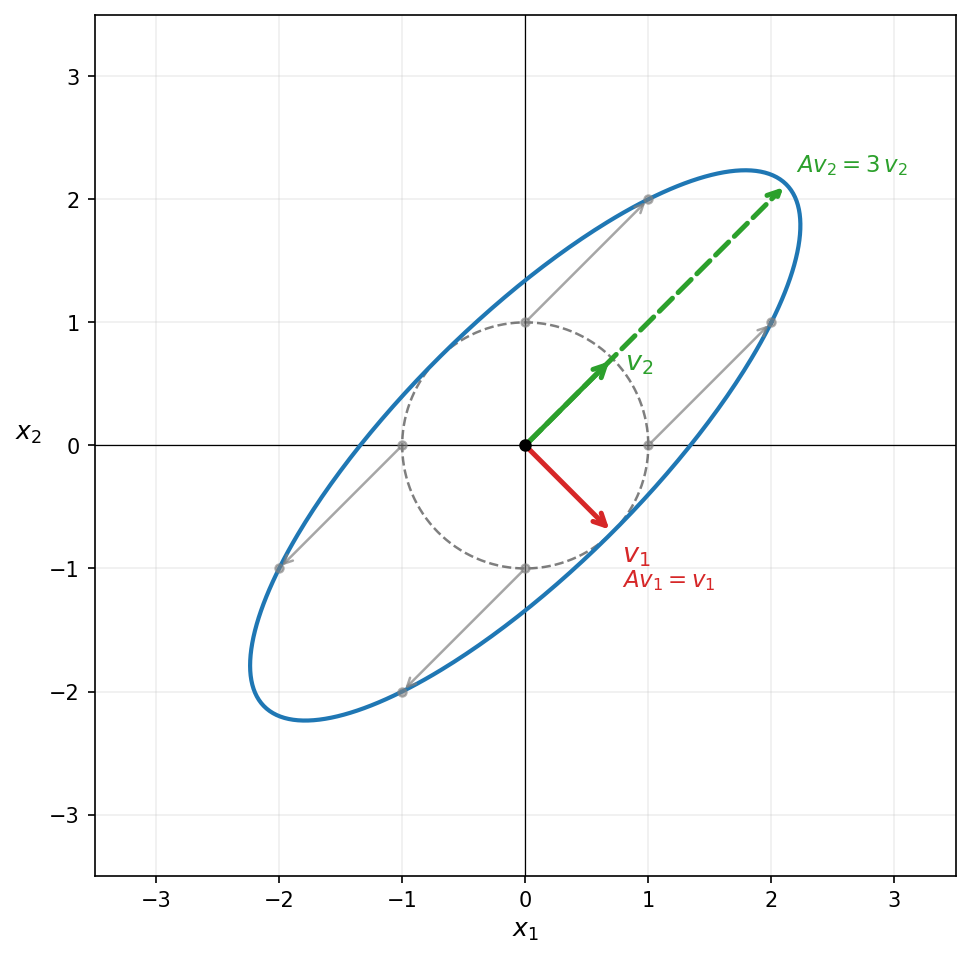
\includegraphics[width=0.68\textwidth]{book/assets/figures/core/fig07_eigenvalues.png}
  \caption{The matrix sends the unit circle to an ellipse. Most directions
  turn. Eigenvector directions are the special directions that only scale.}
\end{figure}

\section{The Shift Test}

The eigenvalue equation can be rewritten as
\[
  (A-\lambda I)v=0.
\]
So $\lambda$ is an eigenvalue precisely when $A-\lambda I$ has a nonzero
kernel.

\begin{proposition}[Eigenvalue as non-invertible shift]
For $A\in\R^{n\times n}$, a scalar $\lambda$ is an eigenvalue of $A$ if and
only if
\[
  \Ker(A-\lambda I)\neq\{0\}.
\]
Equivalently, $A-\lambda I$ is not invertible.
\end{proposition}

\begin{proof}
The equation $Av=\lambda v$ is equivalent to $(A-\lambda I)v=0$. A nonzero
solution exists exactly when the kernel is nontrivial. For a square matrix,
nontrivial kernel is equivalent to non-invertibility.
\end{proof}

For small matrices, one often finds eigenvalues by solving
\[
  \det(A-\lambda I)=0.
\]
This is conceptually useful, but it is not the computational method for large
matrices. Numerical software uses iterative algorithms.

\section{Eigenvectors And Powers}

Eigenvectors matter because repeated application of a linear map is simple
along eigenvector directions.

\begin{proposition}
If $Av=\lambda v$, then for every integer $k\geq 0$,
\[
  A^kv=\lambda^k v.
\]
\end{proposition}

\begin{proof}
Use induction. The case $k=0$ says $I v=v$. If $A^kv=\lambda^k v$, then
\[
  A^{k+1}v=A(A^kv)=A(\lambda^k v)=\lambda^k Av=\lambda^{k+1}v.
\]
\end{proof}

This is why eigenvalues appear naturally in discrete-time dynamics:
\[
  x_{t+1}=Ax_t.
\]
If $x_0$ is an eigenvector, then
\[
  x_t=A^t x_0=\lambda^t x_0.
\]
The direction stays fixed. The magnitude grows if $|\lambda|>1$, decays if
$|\lambda|<1$, and alternates sign if $\lambda<0$.

\section{Diagonalization}

If a basis consists of eigenvectors, then the matrix becomes diagonal in that
basis.

\begin{theorem}[Diagonalization by an eigenbasis]
Suppose $A\in\R^{n\times n}$ has a basis of eigenvectors
$v_1,\ldots,v_n$ with
\[
  Av_i=\lambda_i v_i.
\]
Let
\[
  P=\begin{bmatrix}v_1&v_2&\cdots&v_n\end{bmatrix},
  \qquad
  \Lambda=\diag(\lambda_1,\ldots,\lambda_n).
\]
Then
\[
  AP=P\Lambda,
  \qquad
  P^{-1}AP=\Lambda.
\]
\end{theorem}

\begin{proof}
The $i$-th column of $AP$ is $Av_i=\lambda_i v_i$. The $i$-th column of
$P\Lambda$ is also $\lambda_i v_i$. Hence $AP=P\Lambda$. Since the $v_i$ form
a basis, $P$ is invertible, and multiplying by $P^{-1}$ gives
$P^{-1}AP=\Lambda$.
\end{proof}

\begin{definition}[Diagonalizable]
A square matrix is \emph{diagonalizable} if it is similar to a diagonal matrix:
\[
  P^{-1}AP=\Lambda
\]
for some invertible $P$ and diagonal $\Lambda$.
\end{definition}

Diagonalization is a change of basis. It does not change the linear map; it
finds coordinates in which the map acts by independent scalar multiplications.

\section{Distinct Eigenvalues Give Independent Eigenvectors}

\begin{proposition}
If $u_1$ and $u_2$ are eigenvectors with distinct eigenvalues
$\lambda_1\neq\lambda_2$, then $u_1,u_2$ are linearly independent.
\end{proposition}

\begin{proof}
Suppose $c_1u_1+c_2u_2=0$. Apply $A$:
\[
  c_1\lambda_1u_1+c_2\lambda_2u_2=0.
\]
Subtract $\lambda_1(c_1u_1+c_2u_2)=0$ to get
\[
  c_2(\lambda_2-\lambda_1)u_2=0.
\]
Since $u_2\neq 0$ and $\lambda_2-\lambda_1\neq 0$, we get $c_2=0$. Then
$c_1u_1=0$, so $c_1=0$.
\end{proof}

\begin{corollary}
If $A\in\R^{n\times n}$ has $n$ distinct real eigenvalues, then $A$ is
diagonalizable.
\end{corollary}

Distinct eigenvalues are sufficient, not necessary. The identity matrix has
only one eigenvalue, but every nonzero vector is an eigenvector, so it is
diagonalizable.

\section{A Matrix With Too Few Eigenvectors}

Not every matrix is diagonalizable. Consider the shear-like matrix
\[
  A=\begin{bmatrix}1&1\\0&1\end{bmatrix}.
\]
Solving $Av=v$ gives
\[
  \begin{bmatrix}1&1\\0&1\end{bmatrix}
  \begin{bmatrix}x\\y\end{bmatrix}
  =
  \begin{bmatrix}x\\y\end{bmatrix}
  \quad\Longrightarrow\quad
  y=0.
\]
The eigenspace is the $x$-axis. There is only one eigenvector direction, not a
basis of $\R^2$, so this matrix is not diagonalizable.

\begin{warningbox}
An eigenvalue may repeat without producing enough eigenvectors. Repeated
eigenvalues are not a problem by themselves; the problem is a shortage of
independent eigenvectors.
\end{warningbox}

\section{Dominant Behavior}

Suppose $A$ is diagonalizable and
\[
  x_0=c_1v_1+\cdots+c_nv_n.
\]
Then
\[
  A^t x_0
  =
  c_1\lambda_1^t v_1+\cdots+c_n\lambda_n^t v_n.
\]
If one eigenvalue has largest absolute value and its coefficient is nonzero,
the corresponding eigenvector direction eventually dominates.

This is the core idea behind power iteration, ranking algorithms, stability
analysis, and many iterative methods. The course only needs the introductory
principle: powers of a matrix are hard in standard coordinates, but simple in
an eigenbasis.

\section{Python Thread}

\begin{lstlisting}
import numpy as np

A = np.array([[1.0, 2.0],
              [0.0, 3.0]])

vals, vecs = np.linalg.eig(A)
print("eigenvalues:", vals)

for i in range(len(vals)):
    v = vecs[:, i]
    print(np.allclose(A @ v, vals[i] * v))

# Diagonalization check
P = vecs
Lambda = np.linalg.solve(P, A @ P)   # P^{-1} A P
print(Lambda.round(8))

# Dynamics
x = np.array([2.0, 1.0])
for t in range(5):
    print(t, x)
    x = A @ x
\end{lstlisting}

\begin{labbox}
Lab 8 uses diagonalization to compute matrix powers. Lab 9 later approaches
eigenvalues from the Rayleigh quotient, which is better suited to symmetric
matrices.
\end{labbox}

\section*{Chapter Summary}
\addcontentsline{toc}{section}{Chapter Summary}

\begin{itemize}
  \item Eigenvectors are directions preserved by a linear map.
  \item $\lambda$ is an eigenvalue exactly when $A-\lambda I$ has nonzero
        kernel.
  \item On eigenvectors, powers satisfy $A^kv=\lambda^k v$.
  \item A basis of eigenvectors diagonalizes the matrix.
  \item Distinct eigenvalues give independent eigenvectors, but repeated
        eigenvalues require care.
\end{itemize}

\section*{Exercises}
\addcontentsline{toc}{section}{Exercises}

\subsection*{A. Theory}

\begin{exercise}
\exerciseid{11.A1}
Prove that if $Av=\lambda v$ and $v\neq 0$, then $A^kv=\lambda^kv$ for every
integer $k\geq 0$.
\end{exercise}

\begin{exercise}
\exerciseid{11.A2}
Prove that eigenvectors belonging to two distinct eigenvalues are linearly
independent.
\end{exercise}

\subsection*{B. By Hand}

\begin{exercise}
\exerciseid{11.B1}
Find the eigenvalues and eigenvectors of
\[
  \begin{bmatrix}2&0\\0&3\end{bmatrix}.
\]
\end{exercise}

\begin{exercise}
\exerciseid{11.B2}
For
\[
  A=\begin{bmatrix}1&2\\0&3\end{bmatrix},
\]
verify by hand that $(1,0)^T$ and $(1,1)^T$ are eigenvectors. Build $P$ from
these eigenvectors and compute $P^{-1}AP$.
\end{exercise}

\subsection*{C. Python / NumPy}

\begin{exercise}
\exerciseid{11.C1}
Use \texttt{np.linalg.eig} on a diagonal matrix and on a non-diagonal matrix
with known eigenvectors. Verify $Av=\lambda v$ for each eigenpair.
\end{exercise}

\begin{exercise}
\exerciseid{11.C2}
Choose a diagonalizable $2\times 2$ matrix $A$ and an initial vector $x_0$.
Compute $x_{t+1}=Ax_t$ for $t=0,\ldots,10$ and describe which eigenvector
direction dominates.
\end{exercise}

\subsection*{D. Challenge}

\begin{exercise}
\exerciseid{11.D1}
Give a $2\times 2$ matrix with only one eigenvector direction. Explain why it
cannot be diagonalized.
\end{exercise}

